\chapter{Описание АСУ ТП для СК}\label{ch:chn}

% https://m.studref.com/495961/ekonomika/klassifikatsiya_imitatsionnyh_modeley_promyshlennogo_predpriyatiya

Автоматизированная система управления технологическим процессом (АСУ~ТП) --- это термин,
имеющий отношение к ЭВМ, обеспечивающим управление различными техническими процессами \cite{journal:iter_research_guriev_2016}.
Изначально системы АСУ~ТП использовались исключительно на производстве, но с развитием технологий
и из-за сходства технических процессов АСУ~ТП вышло за рамки управления сугубо производственными процессами
и перешла в другие сферы деятельности, от управления транспортом %\cite{}
до управления техническими процессами зданий \cite{journal:vechisl_tech:2013:Golushko}
и более сложными техническими сооружениями (например, здесь \cite{journal:vechisl_tech:2004_okolnischnikov}).
%
Далее будет показано создание \todo{аналитической} модели объекта контроля
при создании имитатора объекта контроля и его применение на всех этапах жизненного цикла
объекта контроля: от постановки задачи и проектирования системы контроля, до пусконаладочных работ
и сдачи в опытную эксплуатацию.

\section*{Введение}


Стоит отметить, что для более качественной/глубокой имитации необходимо выделять несколько моделей
(которые по факту являются подмоделями, но так как они могут выступать в качестве самостоятельных единиц исследования,
далее будем называть их моделями),
анализируя данные этих моделей (экспериментально) установить свойства этих моделей:
стационарность, детерминированность и проч.

В модели объекта контроля может быть несколько моделей \cite{journal:vechisl_tech:2004_okolnischnikov}:
\begin{itemize}
    \item модель технологического объекта управления (правила перехода);
    \item модель имитации внешних сигналов;
    \item модель внутреннего состояния объекта контроля (токи, напряжения и т.д. и т.п.);
    \item \ldots
\end{itemize}

% Для пояснения смотри рисунок \ref{fig:submodels_asu_tp} и раздел \ref{sec:submodels_asutp}.
% \begin{center}
%     \begin{figure}[hb]
%         % \includegraphics[width=.8\textwidth]{submodels_asu_tp}
%         \caption{\todo{Здесь будут подмодели...}. Структура модели}\label{fig:submodels_asu_tp}
%     \end{figure}
% \end{center}

Поскольку построение чисто аналитической модели имеет недостаток  в виде отсутствия возможности
описать поведение исследуемого объекта во времени, используется имитационная модель.

\textit{Имитационное моделирование} --- процесс построения некоего алгоритма, который имитирует
поведение исследуемого объекта и взаимодействие исходного объекта с учетом возможных случайных входных величин и
воздействий из внешней среды \cite{book:vvedeni_imit_model_1987}.

Объекты контроля, такие как необитаемые автономные подводные аппараты \todo{\ldots},
на которые в любой момент времени возлагается функция готовности к  работе,
нуждаются в проведении проверок при эксплуатации и хранении.
%
Для проверки ОК необходима система контроля. Создание и отладка СК сопряжена со следующими факторами.
%
\begin{itemize}
    \item Дороговизна и труднодоступность достаточного количества статистического материала
    натурных испытаний для отладки алгоритмов ПО СК экономически нецелесообразна, так же связана с риском для жизни испытующих.
    %
    \item ОК находится на этапе проектирования.
    %
    \item Отсутствует возможность подключения к ОК.
    %
    \item Проверка граничных значений алгоритмов ОК, ведущих к разрушению ОК недопустима.
\end{itemize}



\section{Направление информационных потоков} %\label{ch:ch2}

Структурная схема системы контроля показана на рисунке \ref{fig:asc_schema}.
Взаимодействие между каждыми узлами опосредованно, то есть
оператор (диспетчер) взаимодействует с автоматизированным рабочим местом (АРМ),
физическая реализация которого это ЭВМ со специализированным программным обеспечением.
Оператор, выбирая один из режимов работы, сообщает посредством АРМ,
какой набор выходных параметров должна сформировать СК, чтобы объект контроля вышел на заданный режим проверки.
Штрих пунктиром показано взаимодействие оператора с объектом контроля,
которое подразумевает механическое задействование органов управления ОК
или, некий, например, аудио-визуальный контроль состояния узлов ОК.

\begin{center}
    \begin{figure}[hb]
        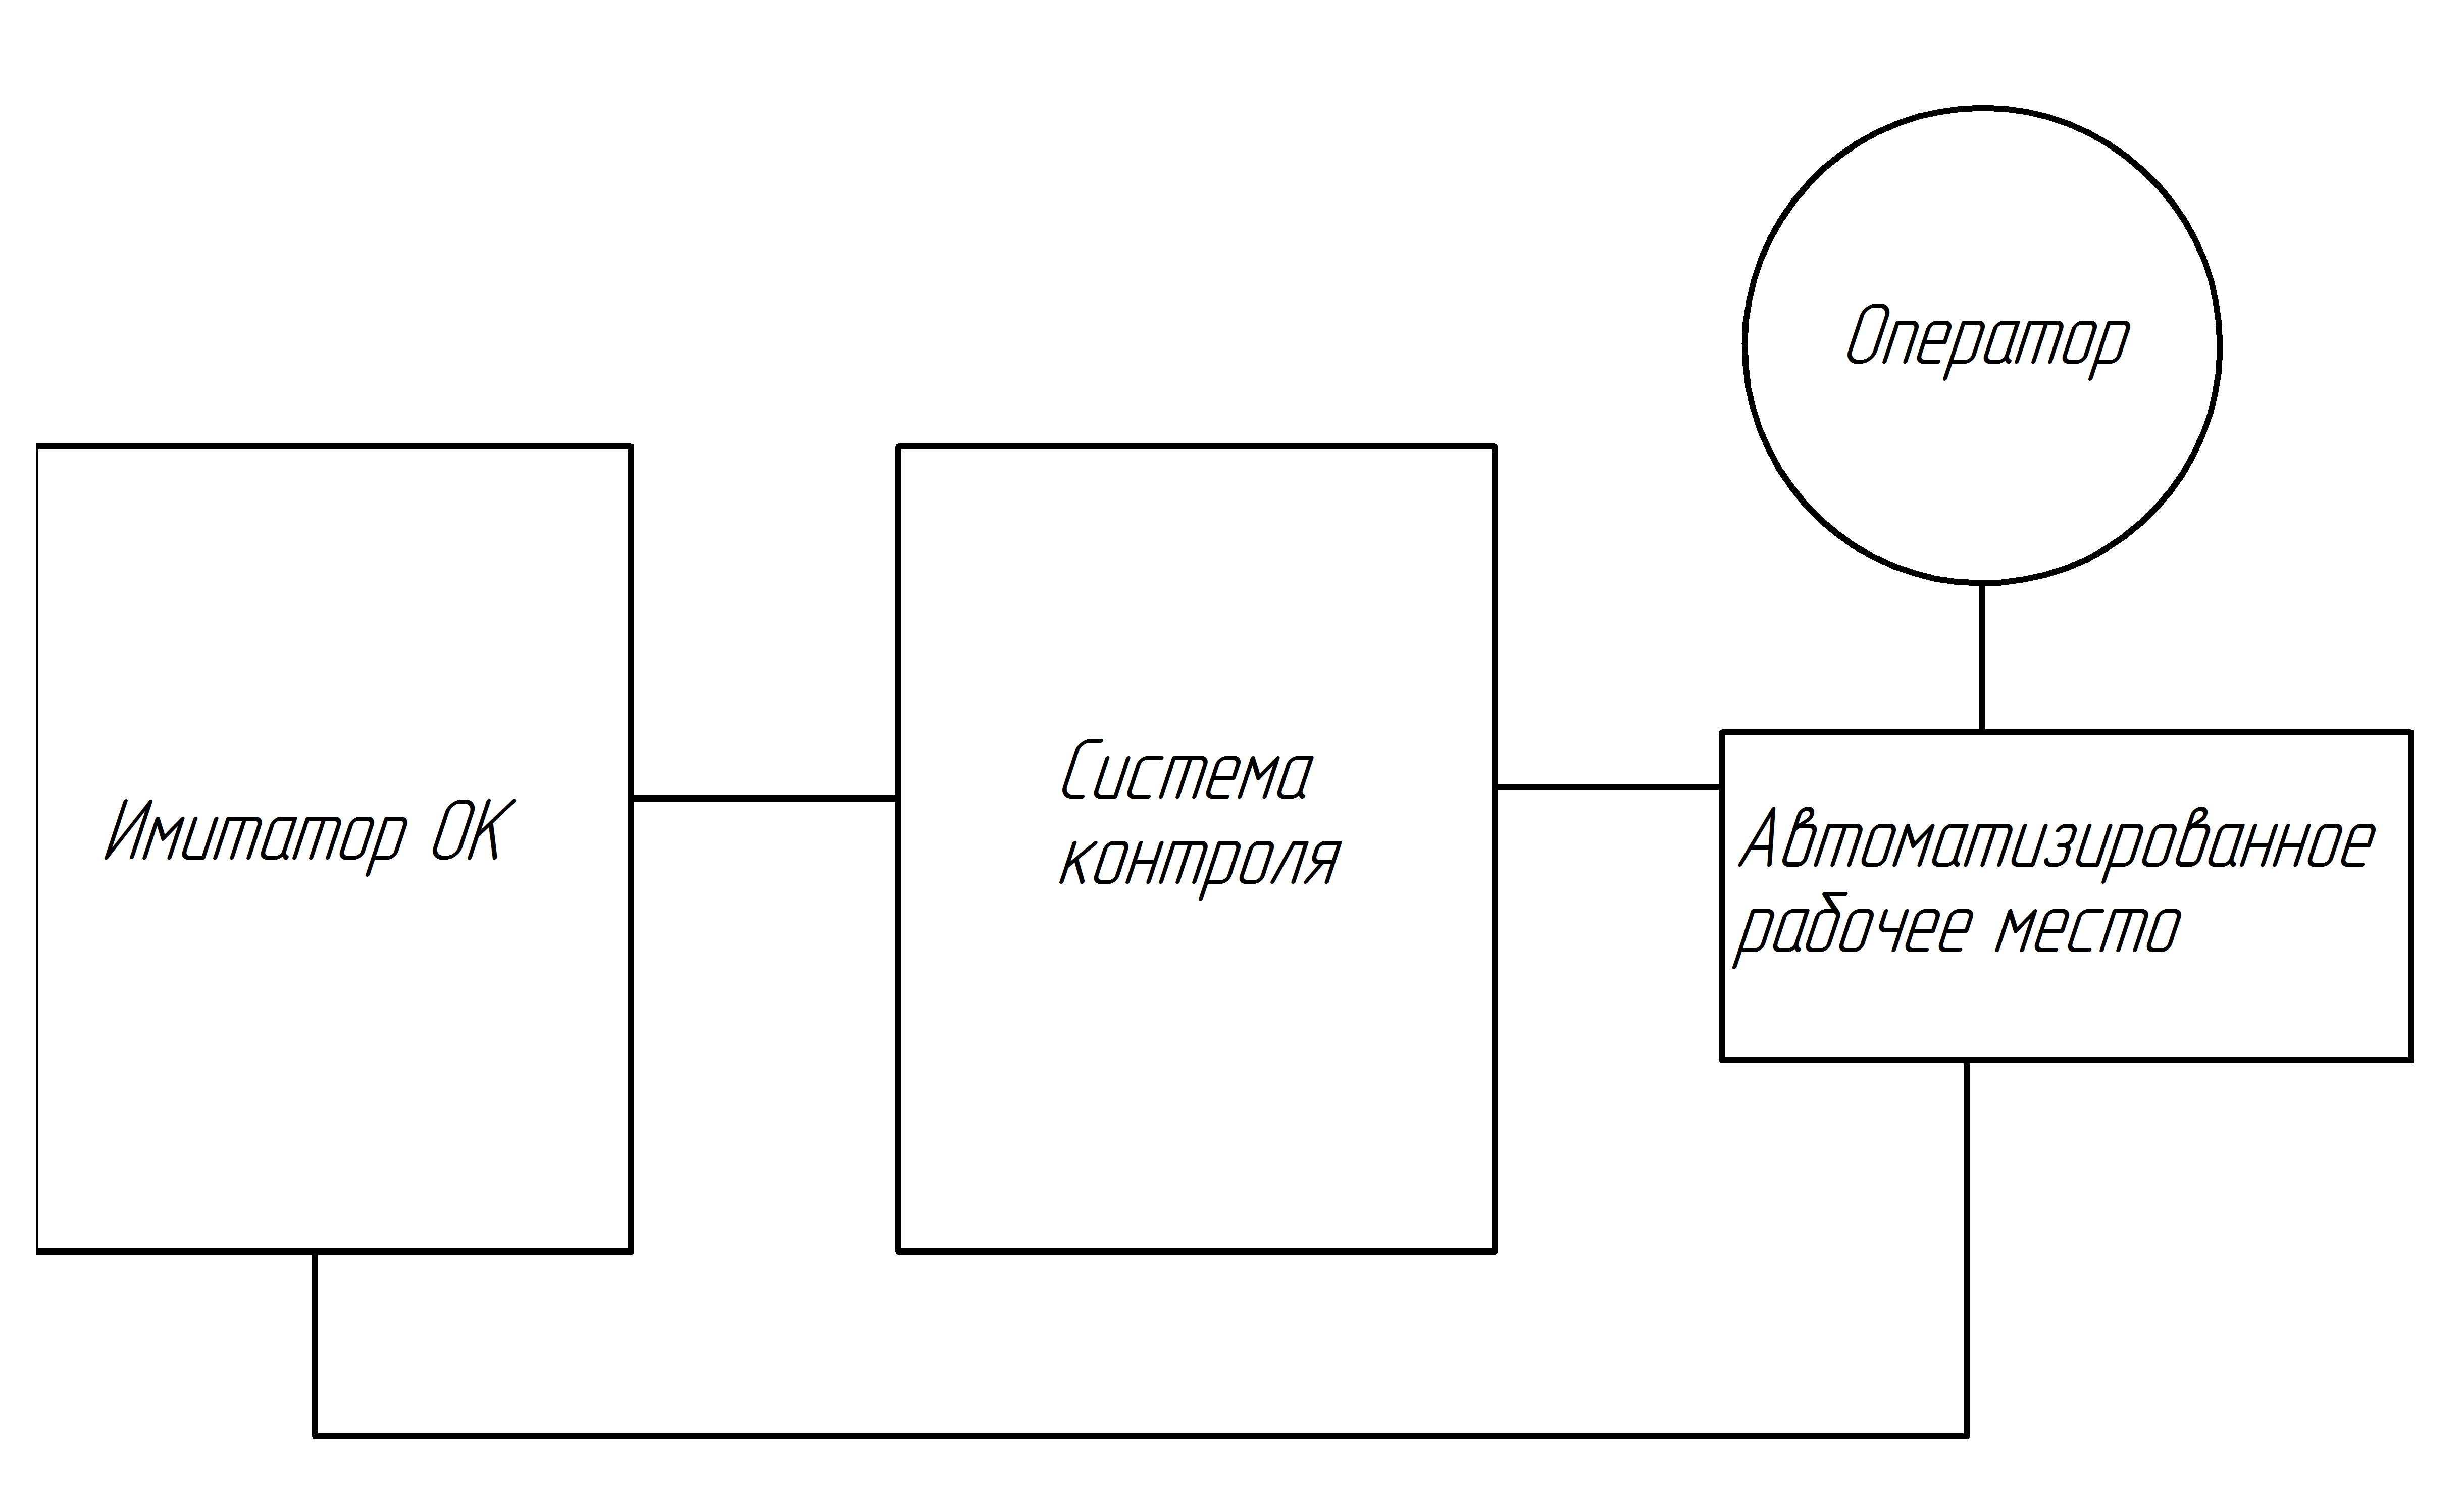
\includegraphics[width=.8\textwidth]{scheme.png}
        \caption{Структура программно-технологического комплекса системы контроля}\label{fig:asc_schema}
    \end{figure}
\end{center}

Более детальное описание информационных потоков показано на рисунке \ref{fig:asc_info_bus}.
Выделяется три уровня: нижний, средний и верхний.

На нижнем уровне располагаются подключаемые по промышленным каналам связи различные приборы, датчики и агрегаты,
которые непосредственно двунаправленно взаимодействуют с ОК, посылая и принимая от него сигналы.
% Так же на этом уровне располагаются прочие устройства, обеспечивающие непосредственное ...

Средний уровень отвечает за обмен информацией между нижним и верхним уровнями. Этот уровень, как правило,
состоит из программируемого логического контроллера (ПЛК). ПЛК реализует различные алгоритмы управления,
осуществляется формирование, сортировка, масштабирование и подготовка данных для передачи между уровнями.
В частности, это может быть осуществлено с помощью блока гальванической развязки (БГР).

Верхний уровень отвечает за графическое представление данных (в широком смысле этого слова),
обеспечивает диспетчеризацию и сбор подготовленных данных посредством человеко-машинного интерфейса.

\begin{center}
    \begin{figure}[hb]
        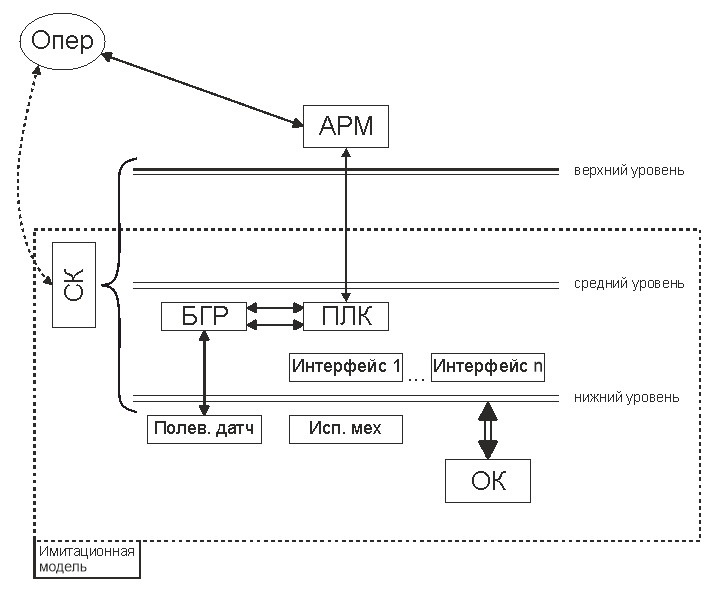
\includegraphics[width=.8\textwidth]{scheme_3levels.png}
        \caption{Информационные шины системы контроля}\label{fig:asc_info_bus}
    \end{figure}
\end{center}

На рисунке \ref{fig:asc_info_bus} штрихом выдела область данных, которая \textit{может быть}
представлена (заменена) имитационное моделью.

Стоит отметить, что в некоторой литературе средний и нижний уровни объединены в один нижний уровень.



\section{Составные части имитационной модели. Контролируемые параметры} \label{sec:submodels_asutp}

Далее обсудим более подробно обмен информацией по промышленному протоколу Modbus.

\subsection{Аналоговые и дискретный стимулы реакции} \label{sect:stimulus_reactions_def}

Множества аналоговых и дискретных реакций
$A^r_{out} = \{a^{r,i}_{out}, i = 1 \dots N^{r,a}_{out}\}$,
$D^r_{out} = \{d^{r,i}_{out}, i = 1 \dots N^{r,d}_{out}\}$,
а так же множества аналоговых и дискретных стимулов
$A^s_{out} = \{a^{s,i}_{out}, i = 1 \dots N^{s,a}_{out}\}$,
$D^s_{out} = \{d^{s,i}_{out}, i = 1 \dots N^{s,d}_{out}\}$
образуют множество параметров $\mathcal{M} = \{A^r_{out}, D^r_{out}, A^s_{out}, D^s_{out}\}$,
передаваемых по сети Modbus. С помощью параметров $m_i \in M$ осуществляется контроль таких параметров,
как: ток потребления, напряжения на силовых установках,
текущая глубина хода, срабатывание различных релейных блоков \todo{\ldots}.

Протокол Modbus позволяет использовать сущности клиент (мастер) и сервер (подчиненный узел)
для организации взаимодействия. В данном случае программа ВУ является клиентом, а ПЛК --- сервером.
Таким образом можно произвести программную имитацию серверной части взаимодействия.
Отождествляя множества стимулов и реакций с протоколом Modbus, мы получаем, что
$D^s_{out}$ соответствуют coils, $A^s_{out}$ -- holding registers,
а $A^r_{out}$,  $D^r_{out}$ -- input registers, discrete inputs, соответственно.

Таким образом получаем множество стимулов $\mathcal{S} = \{D^s_{out}, A^s_{out}\}$
и множество реакций $\mathcal{R} = \{D^r_{out}, A^r_{out}\}$,
причём, $\mathcal{M} = \{\mathcal{R}, \mathcal{S}\} = \mathcal{R} + \mathcal{S}$.

Рассмотрим более подробно какие элементы предметной области
\textit{автономного самоходного подводного аппарата с телеуправлением}
представляются стимулами, а какие -- реакциями.

\subsection{Контролируемые параметры АНПА}

\textbf{Потребная мощность ОК и его составных частей.}
Суммарный ток потребления изделия $I_{tot} = \sum_k^{N_{part}} I_k + \hat I$
и токи контролируемых узлов системы $I_k,\, k\in[1..N_{part}]$,
где $\hat I$ --- ток узлов не подлежащих контролю,
являются аналоговыми реакциями $A^r_{out}$.

Пронумеруем их соответствующим образом $A^r_{out,<i>} = A_i$,
где индекс $i$ пробегает по всем значениям токов,
определённых в техническом задание (тактико-технических характеристиках и проч.) на ОК.

Допустимый диапазон изменений определяется из электрической схемы бортовой сети ОК.
Определим эти диапазоны как константные параметры модели ОК $A_i \in [\min_i, \max_i]$
для каждого контролируемого параметра тока.

Выход $\forall A_i \notin [\min_i, \max_i]$ считается аварийным режимом работы ОК.

\textbf{\todo{
    Выдача определенного напряжения и тока должны происходить при выполнении определенных условий,
    например, таких как инициализация некой заданной программы работы, которая
    отождествляется с набором управляющих стимулов и ответных реакций.
    В принципе, достаточно следить за конечным набором параметров и
    имитировать напряжения и токи моментально или с некой задержкой.
}}

\textbf{Контроль глубины хода изделия.}
Изделие должно следовать на заданной глубине, обусловленной внутренними алгоритмами объекта контроля.
Контроль глубины осуществляется с помощью гидравлической системы,
показания с которой считываются с аналогового датчика глубины (токовый сигнал проходит через БГР).

В общем случае гидравлическая система управляется системой контроля,
по заранее определенному алгоритму, соответствующему выбранному режиму проверки\footnote{Система с обратной связью.}.

\textbf{\todo{
    Таким образом имитация глубины хода ОК производится по заданному сценарию
    после выполнения условий, например, наличие тока потребления
    и на произвольный набор моментов времени $\{t_1, t_2, \ldots, t_n\}$
    происходит изменение глубины $\{h_1, h_2, \ldots, h_n\}$, соответственно.
}}


\textbf{Имитация вращения вала винтов. Пройденная дистанция}
Согласно выбранной программе на ПЛК вырабатывается соответствующая 
частота вращения вала $f_n$ в виде ШИМ сигнала.
Из изделия возвращается сигнал о прохождении определенной дистанции (метка кратного прохождения $m$ метров),
система контроля анализирует интервал времени между передними фронтами меток
и сигнализирует о корректном или некорректном периоде сигналов.
\textbf{\todo{
    Таким образом имитация вращения валов винтов производится выработкой
    прямоугольного сигнала с заданным периодом и скважностью.
}}

Располагая информацией о поступи изделия возможно пересчитать метки $m$ в пройденную дистанцию.
\textbf{\todo{
    Таким образом необходимо иметь возможность генерировать
    сообщения с заданными периодичностью и величиной измениня вещественной переменной
    (в общем случае как на отрицательную, так и на положительную величину).
}}


\textbf{Проводная линия связи.}
Управляющая последовательность битов $b_{in}$, физически представляющая напряжение $|U_{\longrightarrow}|$,
которая имеет следующий вид:
\begin{itemize}
	\item первый бит имеет длительность $\tau^s = s \tau$ с отрицательной полярностью запускающего импульса (ЗИ);
	\item последующие $n$ бит имеют длительность $\tau$
\end{itemize}

\begin{equation} \label{eq:pls_request}
    W_{\longrightarrow} = 
    \overbrace{\mbox{ЗИ}}^{\tau^s}
    \underbrace{000`000`...`00 \overbrace{0}^{\tau}}_{\mbox{$n$ бит}} \,.
\end{equation}

При отрицательной полярности ЗИ, следующий за ним бит имеет противоположную (положительную) полярность.
ЗИ и последовательность бит не имеют пауз между собой.
Отсутствие сигнала между битами более $\delta$ расценивается изделием как логический ноль.

Ответная последовательность бит имеет следующий вид, напряжение ответных сигналов
$|U_{\longleftarrow}| < |U_{\longrightarrow}|$:

\begin{equation} \label{eq:pls_reply}
    W_{\longleftarrow} = 
    \overbrace{\mbox{СИ1}}^{\tau^s}
    \underbrace{000...000}_{\rotatebox{90}{\mbox{Задача}}}
    \overbrace{\mbox{СИ2}}^{\tau^s} \underbrace{000...000}_{\rotatebox{90}{\mbox{Скорость/Курс}}}
    \overbrace{\mbox{СИ3}}^{\tau^s}
    \underbrace{000...000 \overbrace{0}^{\tau}}_{\rotatebox{90}{\mbox{Статус}}}
\end{equation}

СК анализирует наличие трёх синхроимпульсов (СИ), при отсутствии хотя бы одного ответ считается невалидным.
При поступлении трёх невалидных ответов подряд обмен по ПЛС прекращается. 

При проверке анализируется токовый сигнал, при $I_{\mbox{ТУ}\longleftarrow} \geq I_{min}$ бит считается равным логической единице.

Цикл команд (\ref{eq:pls_request}) ответов (\ref{eq:pls_reply}) продолжается до конца выполнения выбранной задачи,
или до досрочной остановки
или до программной имитации обрыва линии связи.

Невыполнение заданной команды управления по ПЛС в течении 
заданного времени $t = k \cdot T$, где
$k$ --- предельно допустимое число сбойных циклов обмена,
$T$ --- длительность полного цикла обмена, считается сбоем работы 
подсистемы ПЛС ОК, при этом ОК должен перейти в автономный режим работы. Контроль продолжается до окончания заложенной программы.

Очевидно, что как ответные последовательности так и управляющие последовательности бит
могут быть преобразованы в многобайтовые слова, которами обменивается ВУ и НУ программного обеспечения СК.
Сериализация и десериализация последовательности бит остается за рамками этой работы,
интерес же представляет обмен непосредственно многобайтовыми словами $W_{\longrightarrow}\,,W_{\longleftarrow}$.

\textbf{\todo{
    Выдача определенного слова должна происходить при выполнении
    конечного множества условий как с задержкой, так и без нее.
}}

\section*{Выводы}

Имитация обмена информацией ПО СК с объектом контроля осуществляется с помощью следующих компонентов:
\begin{itemize}
    \item непосредственная запись значения при выполнении единичного условия;
    \item отложенная запись значения при выполнении единичного условия;
    \item непосредственная запись значения при выполнении множественных условий;
    \item отложенная запись значения при выполнении множественных условий;
    \item периодическое изменение на заданную величину в течении определенного времени.
\end{itemize}
Далее будет показана модель \textit{решающая} эту задачу.

\chapter{По мотивам CIM}

В данном разделе вводится описание конфигурации множества контролируемых параметров,
представленное с помощью конфигурационного файла и использованием расширяемого языка разметки XML, правил его оформления XSD.
Также приводится описание необходимых сущностей для представления
на программном уровне объектов предметной области.


\section{Определение Modbus тегов} \label{sec:modbus_tag}
Пример конфигурационного файла приведен в листинге \ref{lst:modbus_tags_example} в приложении \ref{app:sec:modbus_tag}.
Не смотря на то что в самом протоколе Modbus передаются только целые числа, некоторые производители Modbus-устройств,
в том числе производители средств разработки для программируемых логических контроллеров, расширяют возможности протокола
для передачи вещественных чисел одинарной и двойной точности, так и целочисленных значений размером до восьми байт \cite{book:gost:modbus_program_language}.

Каждый тег описывается тремя обязательными и двумя необязательными аттрибутами.
К обязательным относятся:
\begin{itemize}
    \item[\texttt{title}] заголовок тега, относящийся к предметной области;
    \item[\texttt{address}] адрес тега, согласованный с адресным пространством контроллера;
    \item[\texttt{type}] тип передаваемого значения, который может принимать следующие значения, в зависимости от группы:
    %
    \begin{itemize}
        \item[BOOL] 1 бит;
        \item[WORD] 16 бит;
        \item[DOUBLEWORD] 64 бита;
        \item[REAL] 32 бита;
        \item[LONGREAL] 64 бита.
    \end{itemize}
\end{itemize}
Необязательные аттрибуты служат для вспомогательной цели:
\begin{itemize}
    \item[\texttt{position}] первично -- определяет положение сигнального проводника на модуле в сборке контроллера;
    вторично -- обозначает, что это результат промежуточных вычислений контроллера;
    \item[\texttt{description}] описание передаваемого параметра.
\end{itemize}



\section{Иерархия классов}
На основе анализа предметной области строится иерархия классов для управления информационной моделью,
диаграмма взаимосвязи классов представлена на рисунке \ref{fig:modbus_class_uml} \cite[стр. 223]{book:oop:oop_analize}. 
\begin{landscape}
    \begin{center}
        \begin{figure}[h!]
            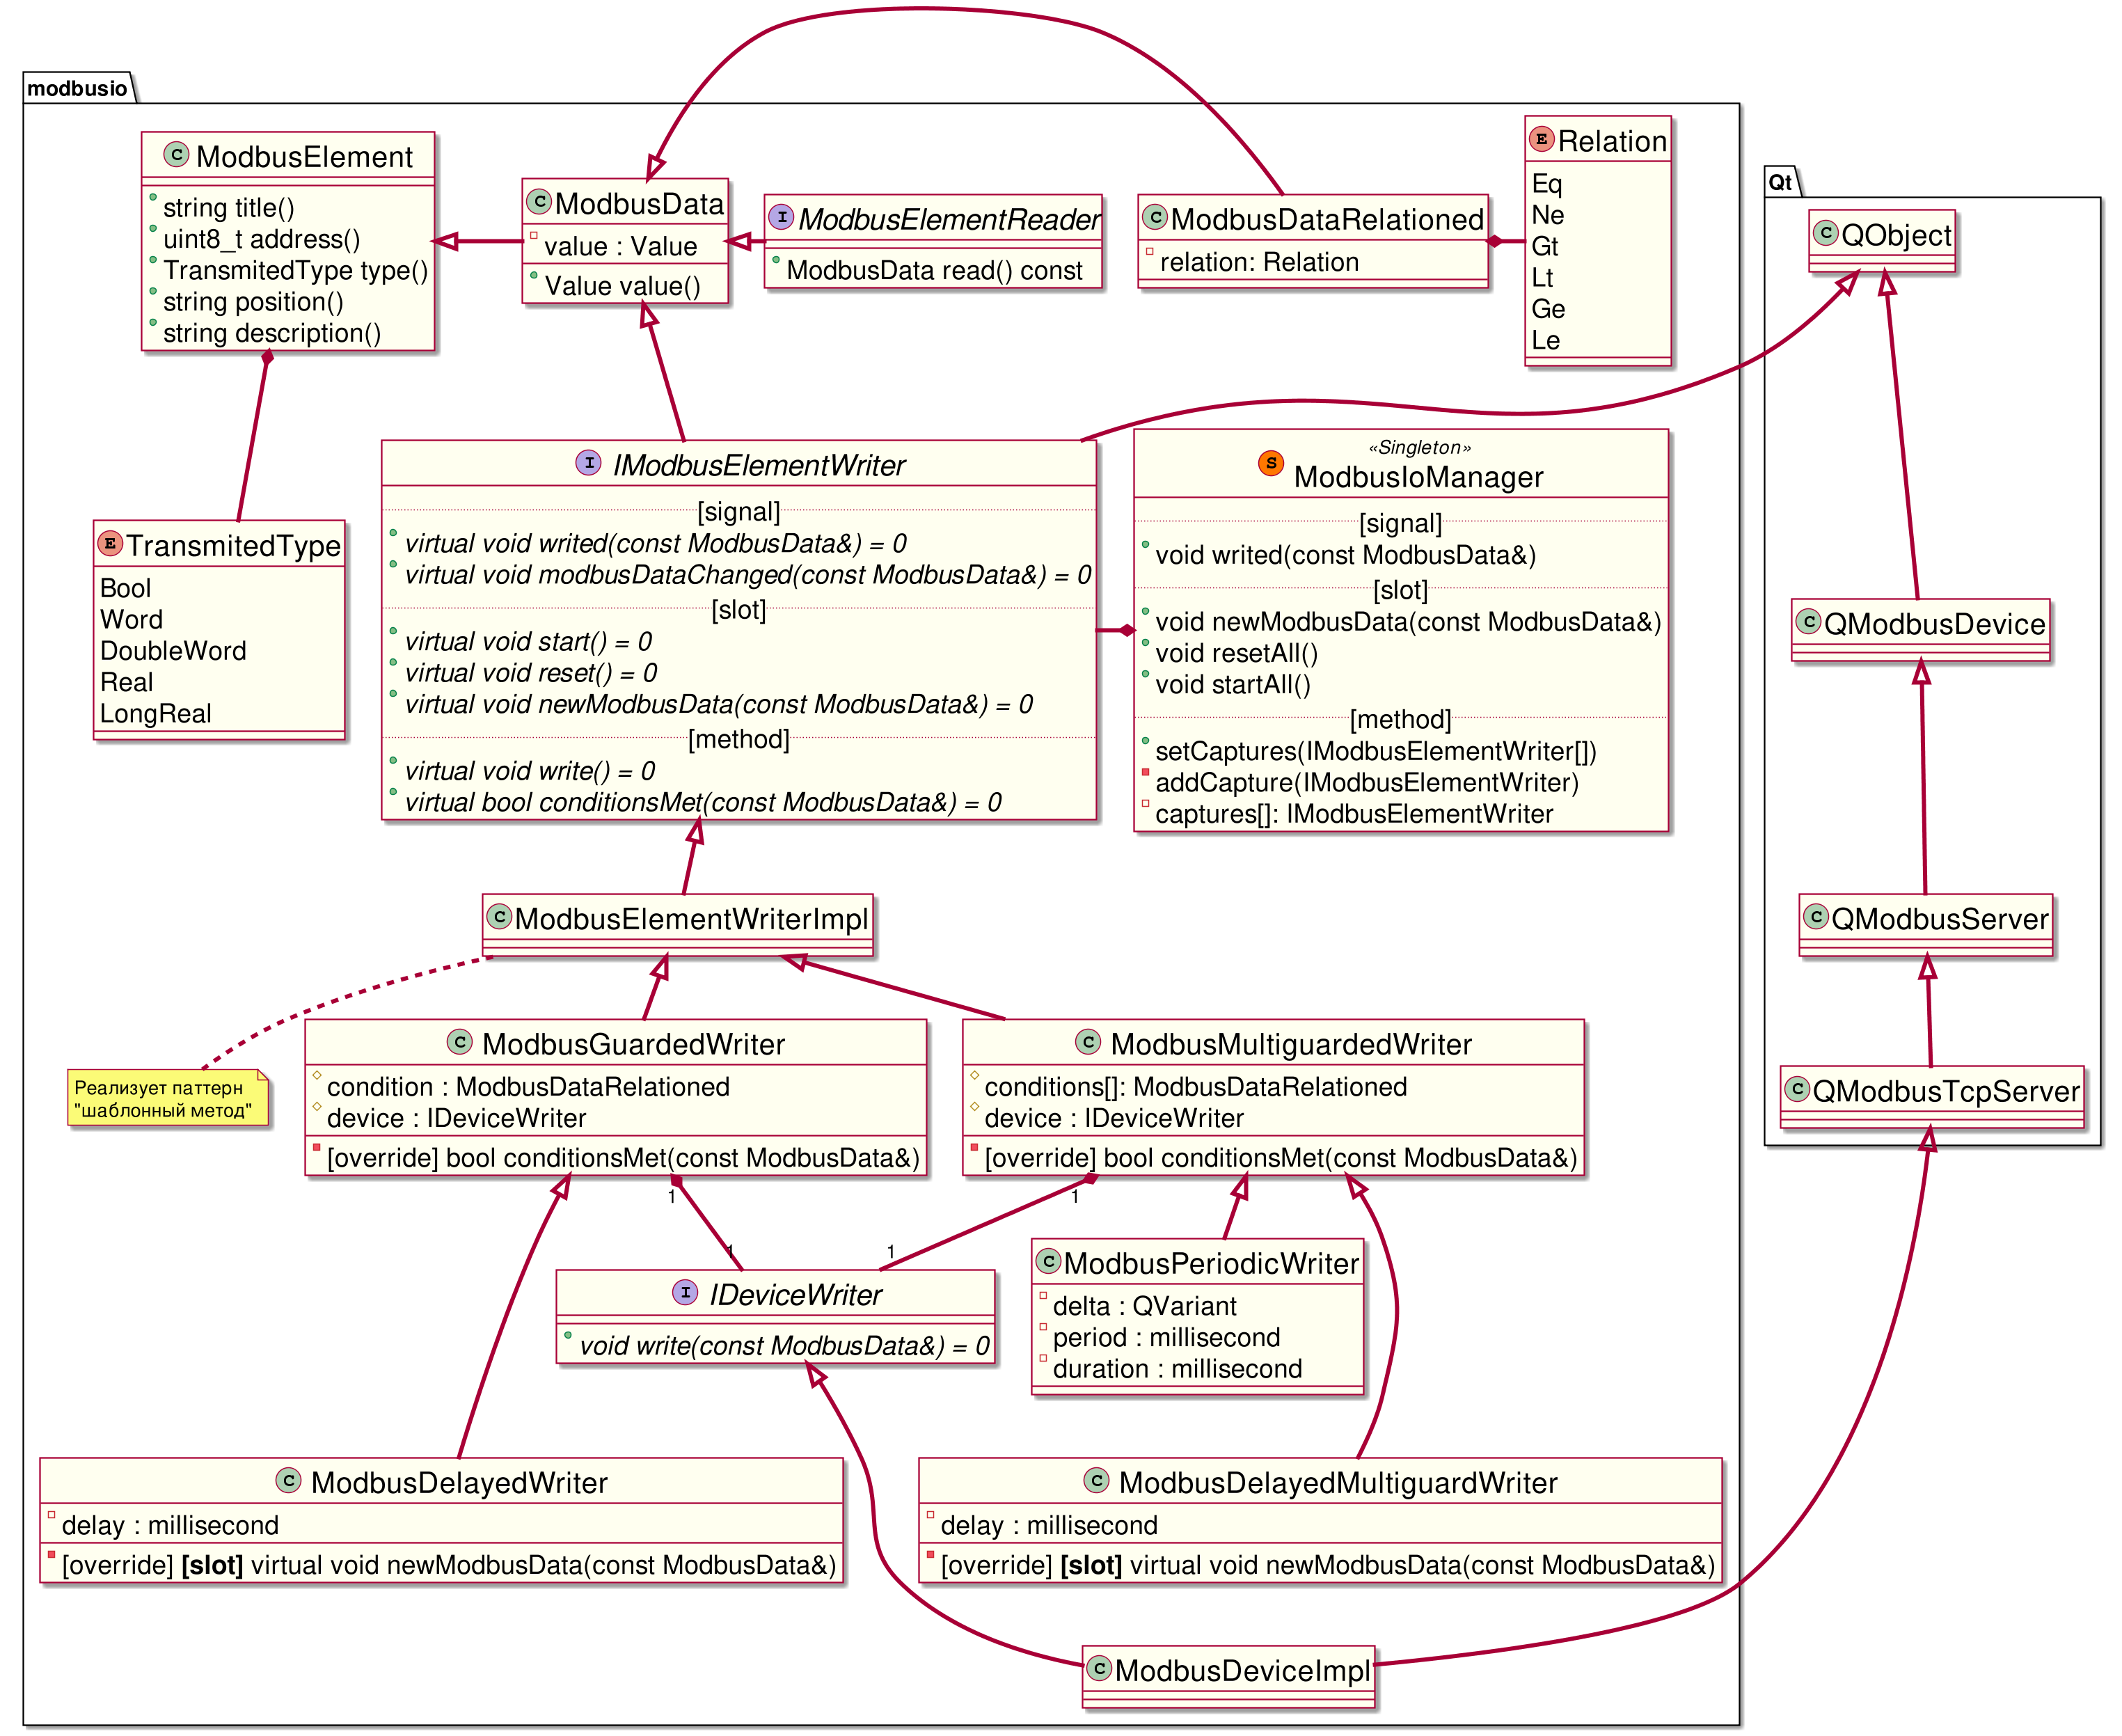
\includegraphics[height=.88\textheight,keepaspectratio]{modbus_class_relationship.png}
            \caption{\todo{UML диаграмма классов для имитатора передачи по сети Modbus}}\label{fig:modbus_class_uml}
        \end{figure}
    \end{center}
\end{landscape}
Базовый класс \texttt{ModbusElement} инкапсулирует в себе представление тега из раздела \ref{sec:modbus_tag}.
Для передачи данных между компонентами системы используется класс \texttt{ModbusData}, производный от \texttt{ModbusElement},
в котором появляется дополнительный член класса \texttt{value} для хранения значения.
Интерфейс \texttt{IModbusElementReader} введен для общности, но в данной работе представляет мало интереса, далее мы сосредоточимся 
на реализациях интерфейса \texttt{IModbusElementWriter}.



\subsection{Жизненный цикл компонента \texttt{IModbusElementWriter}}
Каждый экземпляр класса, реализующего интерфейс \texttt{IModbusElementWriter},
функционирует следующим образом, как показано на рисунке \ref{fig:imodbuselementwriter_activity} \cite[стр. 217]{book:oop:oop_analize}.
После создания, компонент находится в пассивном режиме ожидания, до тех пор пока не будет вызван
метод \texttt{IModbusElementWriter::start()}, после чего компонент подписывается на события шины данных по протоколу Modbus
и слушает сообщения об изменениях значений через слот \texttt{IModbusElementWriter::newModbusData()}.
При поступлении данных, удовлетворяющих условиям функции \texttt{IModbusElementWriter::conditionsMet()},
происходит запись значения через интерфейс \texttt{IDeviceWriter} (рисунок \ref{fig:modbus_device_imp}),
испускается сигнал \texttt{IModbusElementWriter::writed()},
а флаг \texttt{running} выставляется в значение \texttt{false}.
Таким образом, компонент отписывается от событий по шине данных.
Компонент может быть повторно подписан на события, через вызов метода \texttt{IModbusElementWriter::start()}.

\begin{center}
    \begin{figure}
        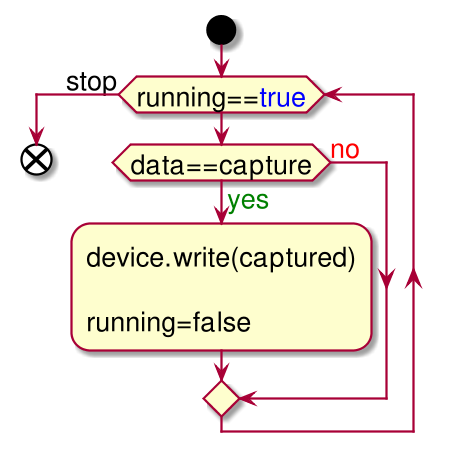
\includegraphics[width=.5\textwidth,keepaspectratio]{imodbuselementwriter_activity}
        \caption{Жизненный цикл компонента (см. также листинг \ref{lst:tmpl_method_writerimpl})}\label{fig:imodbuselementwriter_activity}
    \end{figure}
\end{center}


Класс \texttt{IModbusElementWriterImpl} (не показан на рисунке \ref{fig:modbus_class_uml})
реализует паттерн "Шаблонный метод" (Template method) \cite[стр. 309]{book:pattern:band_of_4},
определяя метод слота \texttt{IModbusElementWriter::newModbusData()}
и защищенный метод \texttt{IModbusElementWriter::write()} --- инвариантную последовательность операций,
определенную виртуальными методами, которые можно переопределить с помощью наследования \cite[стр. 170]{book:tdd:KentBeck}.

\lstinputlisting[
    language=C++,
    caption=Реализация контракта компонента (см. рисунок \ref{fig:imodbuselementwriter_activity}),
    label=lst:tmpl_method_writerimpl
        ]{Dissertation/listings/cpp/writerimpl_template_method.hpp}


\subsection{\todo{Условия перехода}}
Как видно из рисунка \ref{fig:modbus_class_uml} проверка условий записи описываются с помощью компонента типа
\texttt{ModbusDataRelationed} -- наследника класса \texttt{ModbusData}.
Этот класс содержит в себе \texttt{value} от родительского класса и правило отношения \texttt{Relation}.
При поступлении новых данных по шине Modbus происходит сравнение значений (листинг \ref{lst:comparator:compare}).
\lstinputlisting[
    language=C++,
    label=lst:comparator:compare,
    caption=Вспомогательный метод, использующийся при анализе поступающих данных.
        ]{Dissertation/listings/cpp/comparator.hpp}


Перейдем к более подробному рассмотрению реализаций интерфейса \texttt{IModbusElementWriter}.

\subsubsection{Запись с единичным условием}\label{sec:guard}
Циклограмма функционирования класса \texttt{ModbusGuardedWriter} приведена на рисунке \ref{fig:modbus_guarded_writed}.
Этот класс переопределяет метод родительского класса \texttt{IModbusElementWriter::conditionsMet()}.
\begin{center}
    \begin{figure}[h!]
        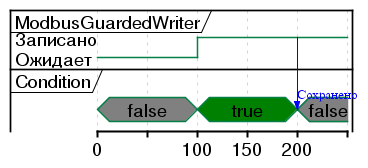
\includegraphics[width=.8\textwidth,keepaspectratio]{modbus_guarded_writer.png}
        \caption{Циклограмма записи значения при выполнении условия в момент времени $\tau_1=100$.}\label{fig:modbus_guarded_writed}
    \end{figure}
\end{center}
Как видно из рисунка выполнение условия происходит в момент времени $\tau_1=100$ условных единиц времени,
сразу же по переднему фронту происходит запись нового значения, которое сохраняется даже после окончания
выполнения логического условия \texttt{cond} в $\tau_2=300$.


\subsubsection{Запись со множественными условиями}
Циклограмма функционирования класса \texttt{ModbusMultiguardedWriter} приведена на рисунке \ref{fig:modbus_multiguarded_writed}.
Этот класс переопределяет метод родительского класса \texttt{IModbusElementWriterImpl::newModbusData()},
так как необходимо следить за множеством тегов через этот слот,
заполняется ассоциативный массив (например, \texttt{std::map<std::string, bool>} у которого ключем является
название тега \texttt{modbusio::ModbusElement::title()}, а значением результат \todo{надо посмотреть в коде \ldots})
\begin{center}
    \begin{figure}[h!]
        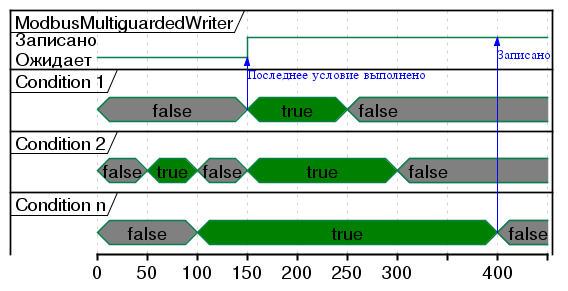
\includegraphics[width=.8\textwidth,keepaspectratio]{modbus_multiguarded_writer.png}
        \caption{Циклограмма записи значения при выполнении множественных условий.}\label{fig:modbus_multiguarded_writed}
    \end{figure}
\end{center}
Как видно из этого рисунка, значение не будет записано до тех пор, пока не будут
выполнены все условия, даже если после установления одного из условий оно меняется
(как показано для второго условия на 100 единице времени). Аналогично с \texttt{ModbusGuardedWriter}
после того как значение было записано, выполнение условий не контролируется, 
при этом записанное значение сохраняется, но может быть независимо изменено по другим причинам,
так как компонент больше не владеет ресурсом и отписывается от событий.


\subsubsection{Отложенная запись с единичным условием}
Циклограмма функционирования класса \texttt{ModbusDelayedWriter} приведена на рисунке \ref{fig:modbus_delayed_writer}.
Этот класс переопределяет метод родительского класса \texttt{ModbusGuardedWriter::conditionsMet()},
при выполнении условия которого запускается таймер на время \texttt{\_delay},
по окончании которого происходит запись значения.
\begin{lstlisting}[language=C++]
    ModbusDelayedWriter::conditionsMet(const modbus::ModbusData& data)
        if (_running && !_timerRun) {
            _timerRun = true;
            QTimer::singleShot(_delay, this, &IModbusElementWriter::write);
        }
\end{lstlisting}

\begin{center}
    \begin{figure}[h!]
        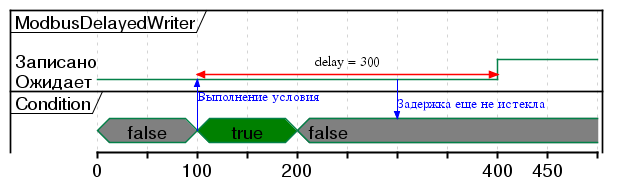
\includegraphics[width=.8\textwidth,keepaspectratio]{modbus_delayed_writer.png}
        \caption{Циклограмма отложенной записи значения при выполнении единственного условия.}\label{fig:modbus_delayed_writer}
    \end{figure}
\end{center}
Класс позволяет устанавливать значение после выполнения условия и по истечению задержки $\tau$.
По окончании таймера на запись значение выражения \texttt{Condition} не анализируется
и запись происходит в любом случае.


\subsubsection{Отложенная запись со множеством условий}
Циклограмма функционирования класса \texttt{ModbusDelayedMultiguardWriter} приведена на рисунке \ref{fig:modbus_delayed_multiguarded_writer}.
\todo{Надо посмотреть код, чтобы точно сказать какой метод переопределен \ldots}
\begin{center}
    \begin{figure}[h!]
        \includegraphics[width=.8\textwidth,keepaspectratio]%
            {modbus_delayed_multiguarded_writer.png}
        \caption{Циклограмма отложенной записи значения при выполнении множественных условий.}\label{fig:modbus_delayed_multiguarded_writer}
    \end{figure}
\end{center}


\subsubsection{Периодическая запись}
Данный компонент предназначен для реализации периодических событий, как показано на диаграмме \ref{fig:modbus_periodic_writer}.
При захвате управления дискретной переменной, ее значение инвертируется каждый период
$f_i(x; \tau) = \lnot f_{i-1}(x; \tau), f(x; \tau) \in \{True, False\}$
(на графике сверху захвачен булевский тег, период равен 25 единиц времени).
При захвате вещественной переменной значение меняется по закону
$f_i(x,\Delta x; \tau) = f_{i-1}(x,\Delta x; \tau) + \Delta x, \Delta x \in \mathcal{R}$
(на графике снизу период равен 50 единиц времени, $\Delta x = 10$ на 200 единиц времени).
\begin{center}
    \begin{figure}[h!]
        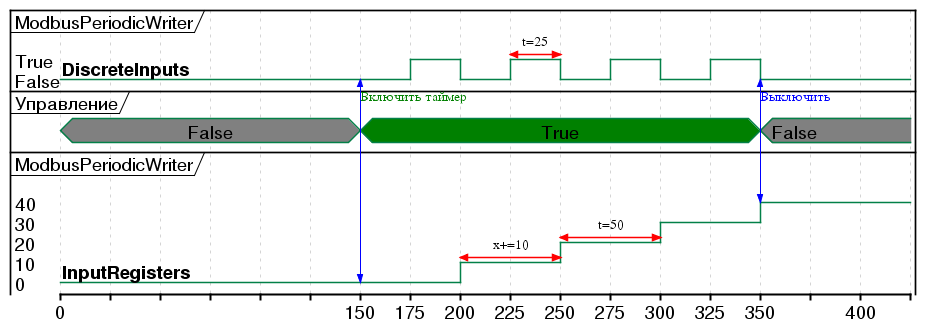
\includegraphics[width=.8\textwidth,keepaspectratio]{modbus_periodic_writer.png}
        \caption{Циклограмма периодической записи значения.}\label{fig:modbus_periodic_writer}
    \end{figure}
\end{center}
Этот компонент используется, например, для управления значениями количества оборотов,
количества транзакций и пакетов, переданных от контроллера к программе верхнего уровня,
при захвате вещественных переменной.
Очевидно, что приращение $\Delta x$ может быть как положительным, так и отрицательным.

Если в конфигурации сценария (листинг \ref{lst:modbus_periodic_writer_xml}) имеется аттрибут
\texttt{duration}, компонент будет работать от выполнения условий до окончания указанной длительности.
В противном случае обновление значений будет происходить до момента прекращения работы
\texttt{ModbusIoManager::resetAll()}.


\subsection{Реализация интерфейса \texttt{IDeviceWriter}}
При реализации интерфейса \texttt{IDeviceWriter} используется возможность множественного наследование языка программирования \cpp,
одним из родителей является интерфейс \texttt{IDeviceWriter},
а вторым --- класс библиотеки \texttt{Qt}, обеспечивающий реализацию физической передачи информации по протоколу Modbus
\texttt{QModbusTcpServer}, так как обмен происходит по разновидности протокола Modbus TCP/IP.
Упрощенная реализация показана в листинге \ref{lst:imodbus_device_impl}.
\begin{center}
    \begin{figure}
        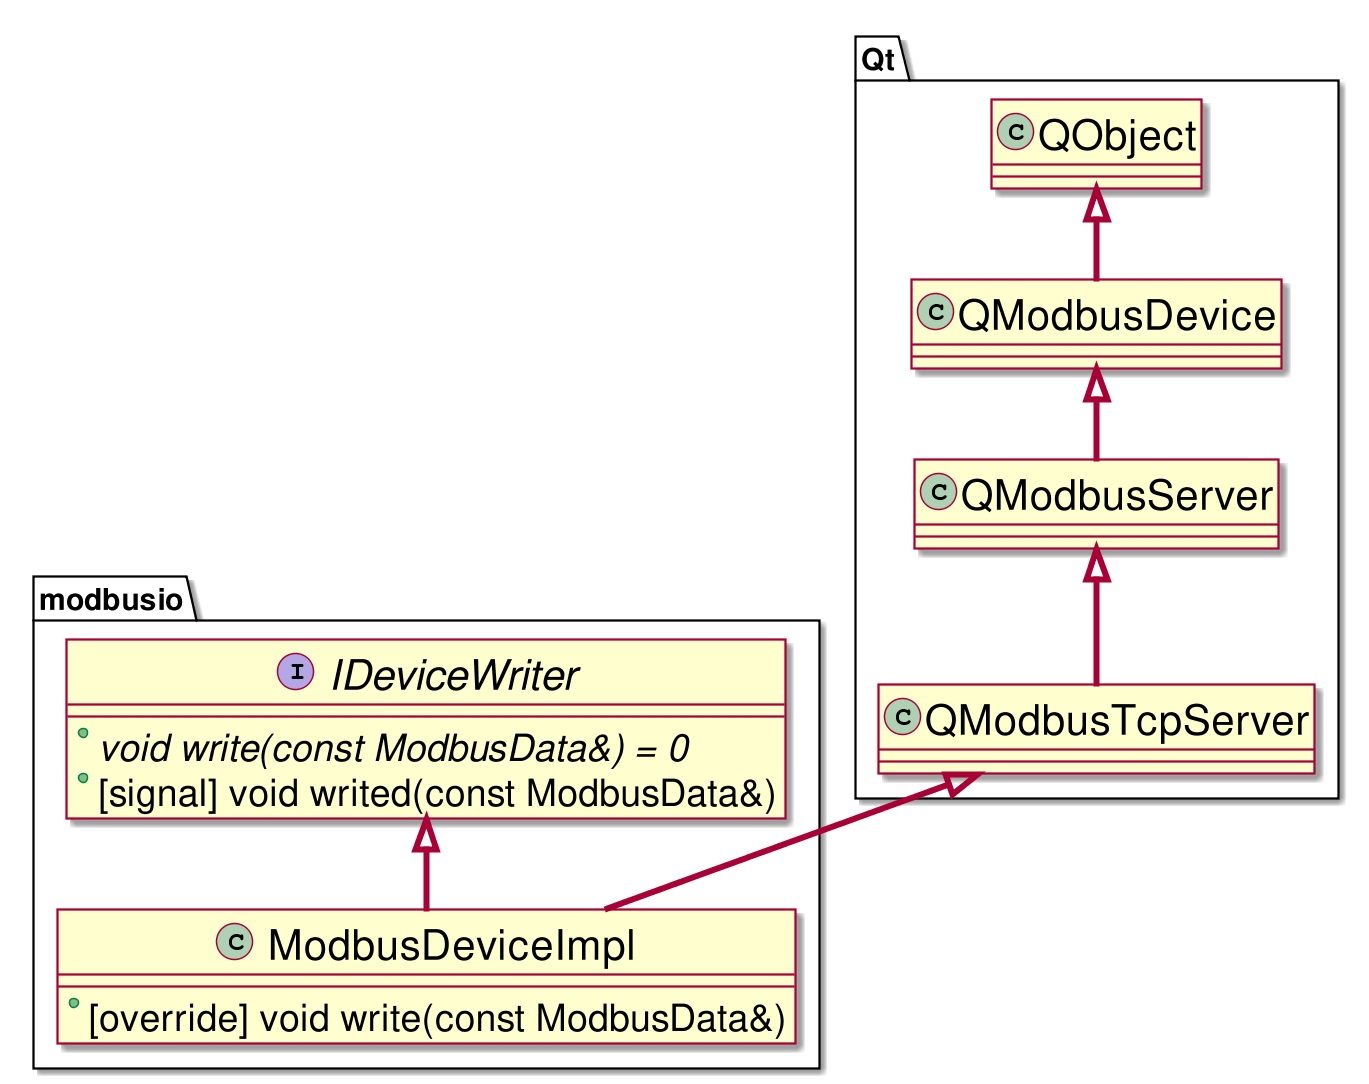
\includegraphics[width=.9\textwidth,keepaspectratio]{modbus_device_impl.png}
        \caption{Реализация устройства для записи значений по протоколу Modbus}\label{fig:modbus_device_imp}
    \end{figure}
\end{center}
\lstinputlisting[
    language=C++,
    caption=Простейшая реализация \texttt{IDeviceWriter} устройства,
    label=lst:imodbus_device_impl]
        {Dissertation/listings/cpp/dummydeviceimpl.hpp}
Таким образом используется интерфейс вместо конкретной реализации \cite[стр. 47-48]{book:pattern:head_first}


\subsection{Описание конфигурационного файла для компонентов интерфейса \texttt{IModbusElementWriter}}
Каждая группа должна быть помещена в корневой элемент \texttt{Scenario},
как показано в листинге \ref{lst:modbus_scenario_example_diagram} приложения \ref{app:sec:modbus_scenario_example_diagram}.

Каждый компонент помещается внутри тега \texttt{Writer},
с обязательным текстовым аттрибутом \texttt{tag}, который указывает каким ресурсом владеет данный компонент
и обязательным аттрибутом \texttt{value}, который выполняет различную роль в зависимости от назначения компонента (см. листинг \ref{lst:modbus_tags_scenario_configs}).
Одновременно владеть одним и тем же ресурсом могут несколько компонентов (как будет показано ниже).
Далее следует секция условий, которая присутствует даже для компонентов \texttt{ModbusGuardedWriter} и \texttt{ModbusDelayedWriter},
для общности парсера конфигурационного файла.
Каждое условие описывается логической операцией отношения \texttt{relation} для смежного параметра, указанного в обязательном поле \texttt{tag} и
связанного с ним значения \texttt{value}.
Элемент \texttt{relation} принимает одно из следующих значений:
\texttt{eq} ($=$),
\texttt{ne} ($\neq$),
\texttt{gt} ($>$),
\texttt{lt} ($<$),
\texttt{ge} ($\geq$),
\texttt{le} ($\leq$), по аналогии с обозначениями в языке Fortran.
Для дискретных (булевых) переменных необязательно указывать отношения типа \texttt{eq},
если интересует отношение равенства, отношение \texttt{ne} неравенства же необходимо указывать явным образом.
Необязательным полем является поле \texttt{Description}, в котором размещается информация для
обозначения назначения компонента в сценарии, а так же могут располагаться другие произвольные текстовые данные.

\subsubsection{ModbusGuardedWriter}
Рассмотрим более подробно описание компонента для компонента с единичным условием записи,
который размещается в элементе \texttt{Guarded}:
\lstinputlisting[
    language=MyXML,
    caption=Пример конфигурации \texttt{ModbusGuardedWriter},
    label=lst:modbus_guarded_writer_xml]
        {Dissertation/listings/xml/guarded.xml}
Захватывается управление над тегом \texttt{A1}, которой будет присвоено значение 160
при выполнении условия \texttt{R1 = true}.


\subsubsection{ModbusMultiguardedWriter}
Для описания компонента со множественными условиями, используется следующий формат,
который размещается в элементе \texttt{Multiguarded}:
\lstinputlisting[
    language=MyXML,
    caption=Пример конфигурации \texttt{ModbusMultiguardedWriter},
    label=lst:modbus_multiguarded_writer_xml]
        {Dissertation/listings/xml/multiguarded.xml}
Переменной \texttt{Regime} будет присвоено значение 1, как только 
одновременно будет выполнено два условия: $Regime = 1: \{A1 \ge 150 \wedge C1 = true\}$.

\subsubsection{ModbusDelayedWriter и ModbusDelayedMultiguardWriter}
Компоненты этого типа располагаются в окружении тегов элементов \texttt{Delayed} и \texttt{Multidelayed}, соответственно.
\lstinputlisting[
    language=MyXML,
    caption=Пример конфигурации \texttt{ModbusDelayedWriter} и \texttt{ModbusDelayedMultiguardWriter},
    label=lst:modbus_delayed_writer_xml]
        {Dissertation/listings/xml/delayed.xml}
Захватывается управление переменной \texttt{PP\_1}, которой будет установлено значение \texttt{true}
через 50 единиц времени, как только будут выполнены два условия:
$PP\_1 = \mbox{true}: \{R1 = true \wedge A1 \le 150\}$.


\subsubsection{ModbusPeriodicWriter}
Данный компонент располагается внутри элемента \texttt{Period} в конфигурационном файле сценария.
\lstinputlisting[
    language=MyXML,
    caption=Пример конфигурации \texttt{ModbusPeriodicWriter},
    label=lst:modbus_periodic_writer_xml]
        {Dissertation/listings/xml/periodic.xml}
В данном примере дистанция, ассоциированная с переменной \texttt{Distance}, увеличивается на 100 единиц каждые 1000 единиц времени,
при выполнении ряда условий, а именно: $\{C1 = true \wedge A1 > 100 \wedge A1 \le 150 \}$ или
увеличивается на теже 100 единиц, но с периодом 500 единиц, когда достигаются следующие условия:
$\{C1 = true \wedge A1 > 150\}$
Отметим, что для этого компонента начальное значение устанавливается с помощью аттрибута \texttt{value}
при вызове метода \texttt{IModbusElementWriter::start()}.


\subsection{Сводная таблица наследников \texttt{IModbusElementWriter}}
\begin{table}[]
\caption{\todo{Сводная таблица наследников}}\label{tbl:IModbusElementWriterImpl}
\begin{tabular}{|l|c|c|c|c|c|c|c|c|}
\hline
    \multicolumn{1}{|c|}{\multirow{2}{*}{Наследники}} &
    \multicolumn{6}{c|}{\textbf{Аттрибуты}} &
    \multicolumn{2}{c|}{\textbf{Переопределенные методы наследника}} \\ \cline{2-8} 
    \multicolumn{1}{|c|}{}     &
        \rotatebox{90}{tag} & \rotatebox{90}{value}  & \rotatebox{90}{delay}  & \rotatebox{90}{period} &
        \rotatebox{90}{delta} & \rotatebox{90}{duration} &
        \rotatebox{90}{conditionsMet} & \rotatebox{90}{newModbusData} \\ \hline
    \texttt{ModbusGuardedWriter}              & +    & +      & -      & -      & - &-     & + & -  \\ \hline
    \texttt{ModbusMultiguardedWriter}         & +    & +      & -      & -      & - &-     & + & -  \\ \hline
    \texttt{ModbusDelayedWriter}              & +    & +      & +      & -      & - &-     & - & +  \\ \hline
    \texttt{ModbusDelayedMultiguardWriter}    & +    & +      & +      & -      & - &-     & - & +  \\ \hline
    \texttt{ModbusPeriodicWriter}             & +    & +      & -      & +      & + &$\pm$ & + & -  \\ \hline
\end{tabular}
\end{table}


\subsection{Менеджер состояний}
Для управления компонентами имитатора используется менеджер \texttt{ModbusIoManager}. Установка компонентов производится с помощью экземпляра класса \texttt{ScenarioParser}, реализующего интерфейс \texttt{IParser}.
Этот интерфейс является общим для как для чтения файла сценария (\ref{lst:modbus_scenario_example_diagram}),
так и для файла тегов (листинг \ref{lst::modbus_tags_example}).
После чтения конфигурации, ее необходимо проверить, что каждый тег $t_i$
компонента, управление над которым захватывает и условия выполнения переходов, является элементов множества \texttt{ModbusTags},
то есть $\forall t_i \in \mbox{ModbusTags}$.
\begin{center}
    \begin{figure}
        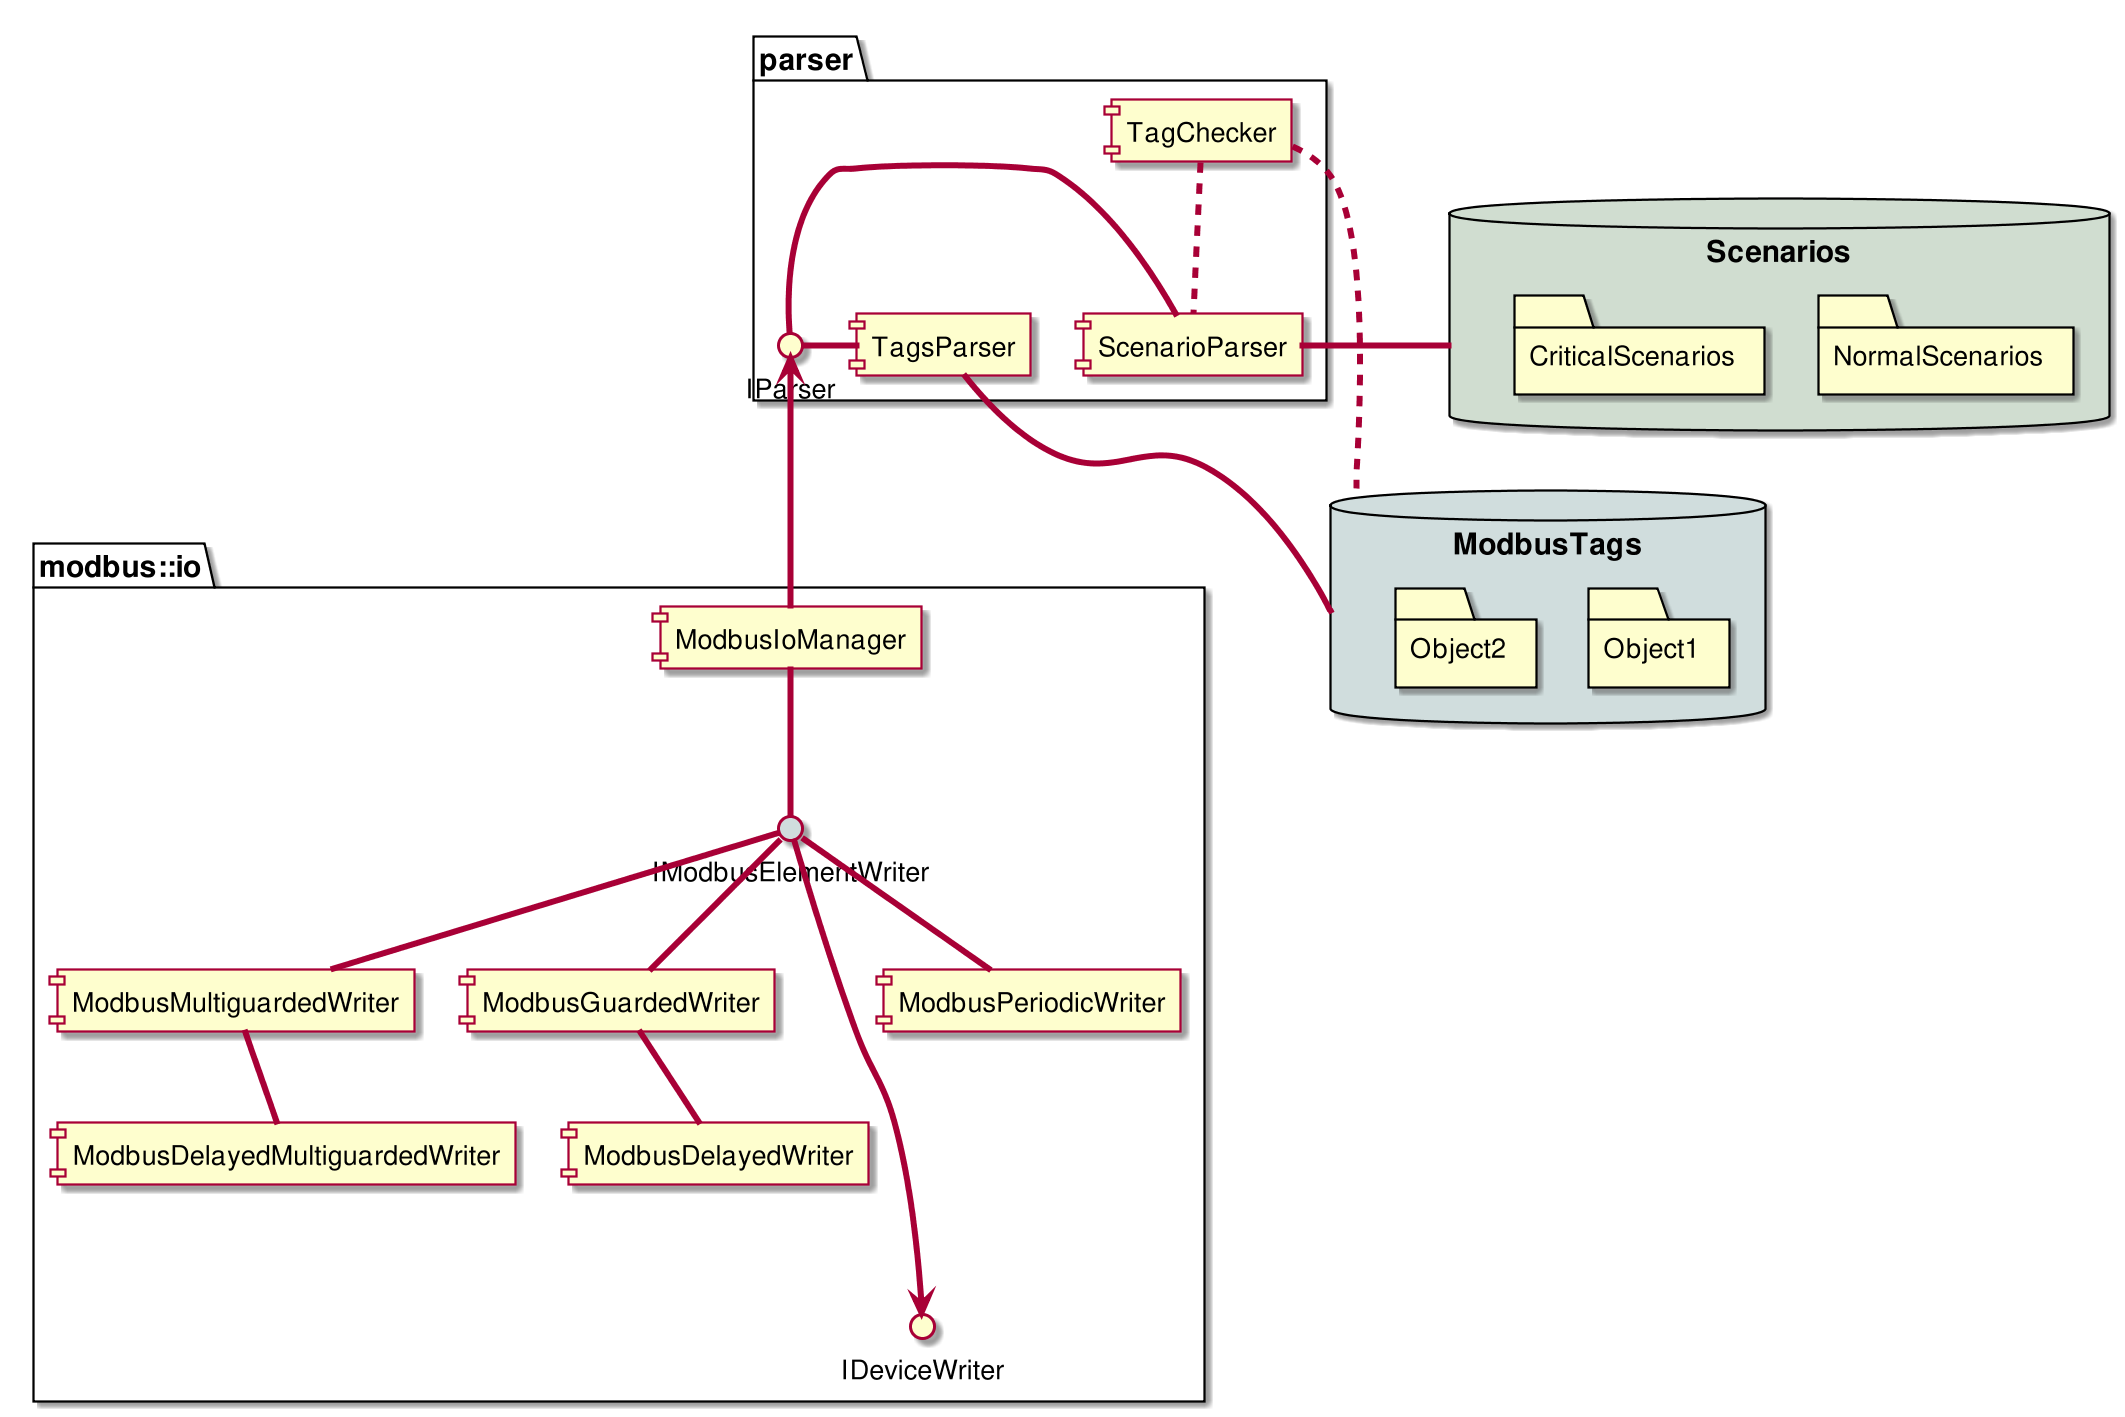
\includegraphics[width=.9\textwidth,keepaspectratio]{modbus_class_components}
        \caption{Композиция классов менеджера сценариев}\label{fig:modbus_class_components}
    \end{figure}
\end{center}

\begin{center}
    \begin{figure}
        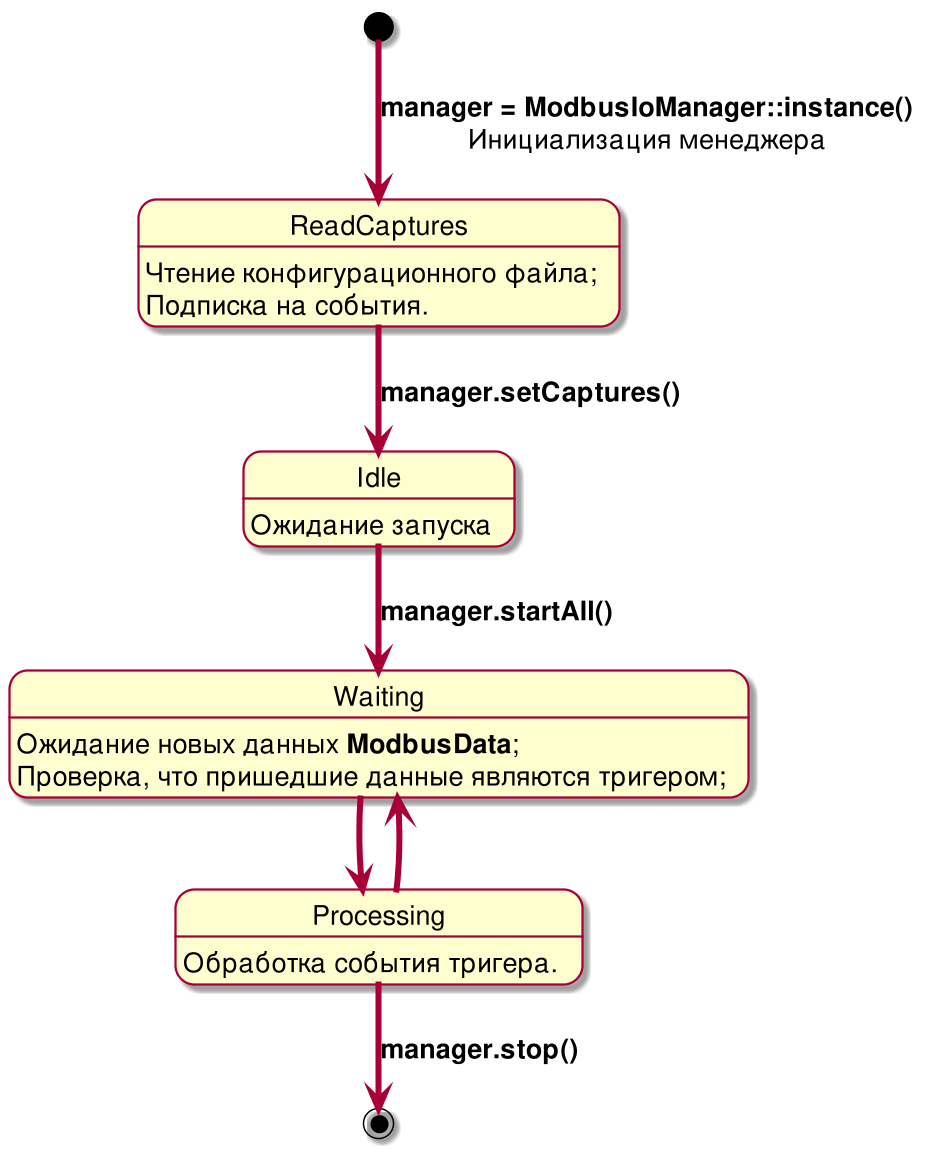
\includegraphics[width=.9\textwidth,keepaspectratio]{modbusiomanager_state_diagram}
        \caption{\todo{Жизненный цикл ModbusIoManager}}\label{fig:modbusiomanager_state_diagram}
    \end{figure}
\end{center}

Последовательность действий показана на рисунке \ref{fig:top_level_sequence} \cite[стр. 239]{book:oop:oop_analize}
\begin{center}
    \begin{figure}
        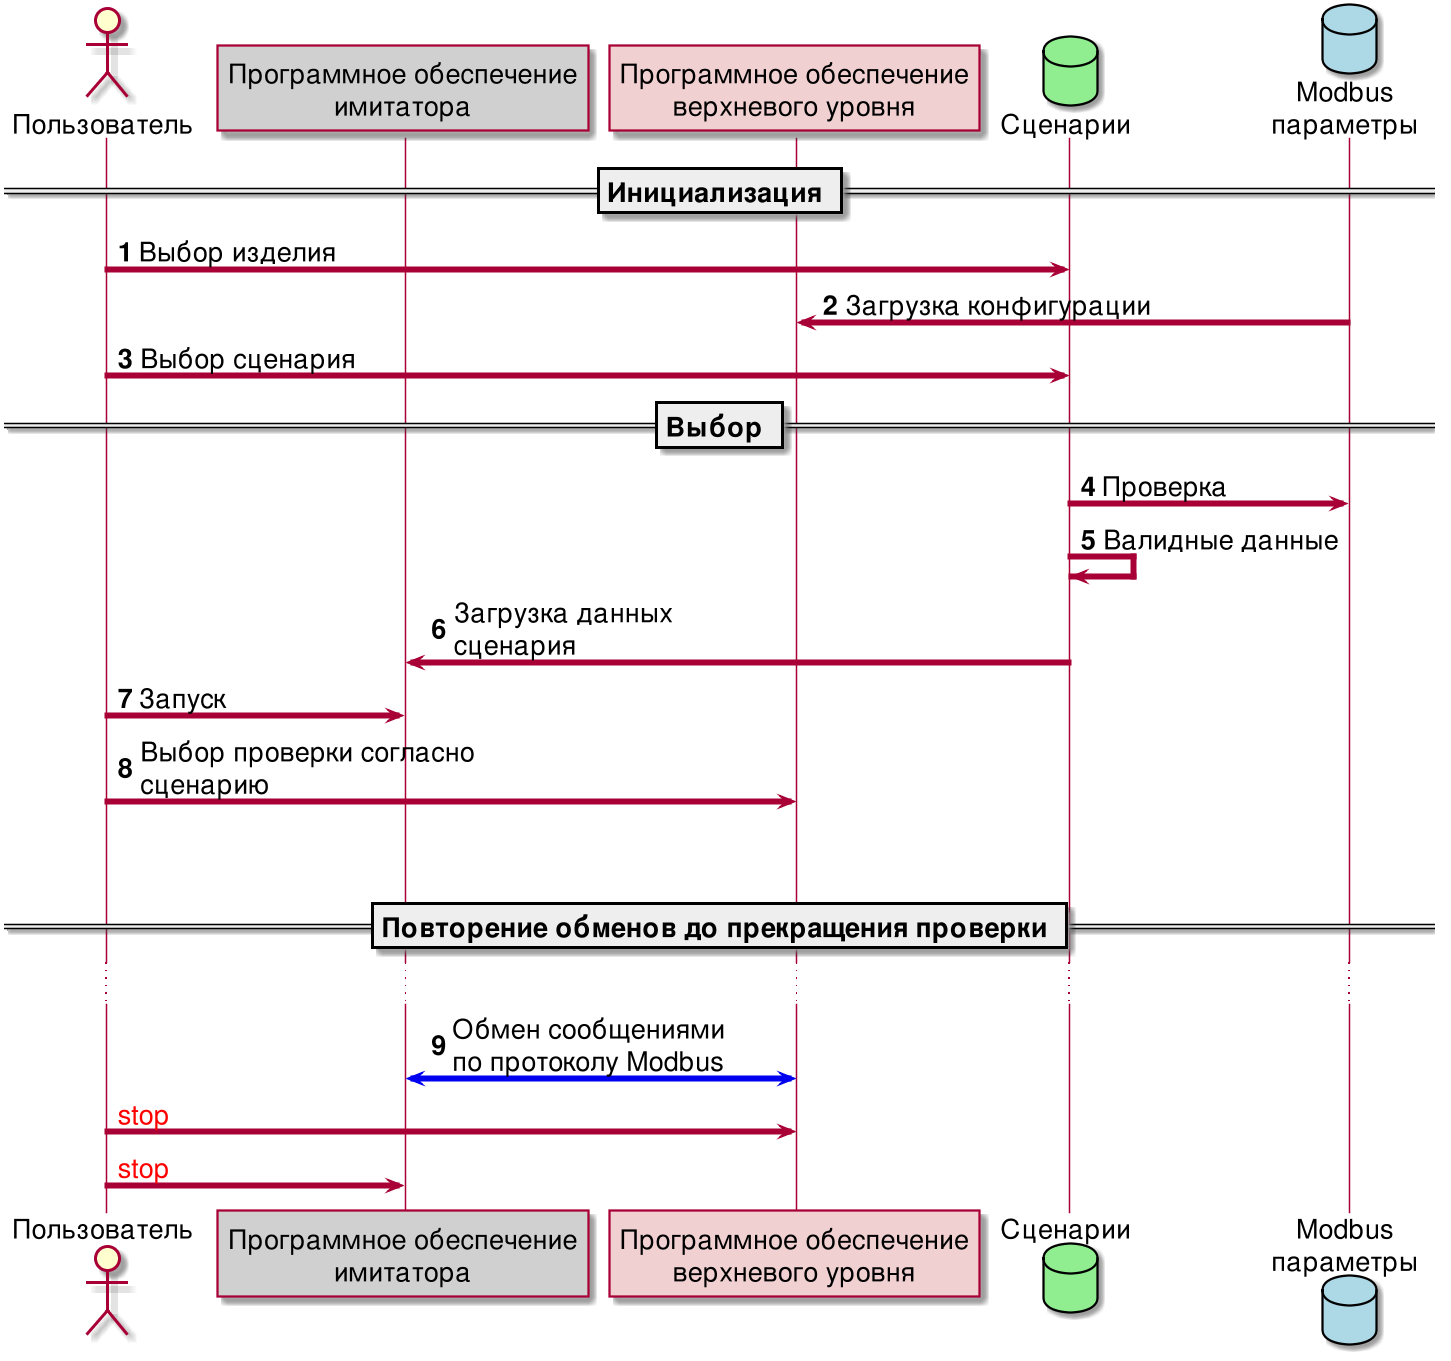
\includegraphics[width=.9\textwidth,keepaspectratio]{top_level.png}
        \caption{Последовательность действий при работе с имитатором}\label{fig:top_level_sequence}
    \end{figure}
\end{center}

\clearpage
\section{Пример композиции для простейшего сценария}

Рассмотрим пример сценария на основе множества Modbus тегов из листинга \ref{lst:modbus_tags_example},
циклограмма которого представлена на рисунке \ref{fig:modbus_scenario_example_diagram},
сценарий приведен в листинге \ref{lst:modbus_scenario_example_diagram} в разделе приложения \ref{app:sec:modbus_scenario_example_diagram}.
% Схема разметки приведена в листинге \ref{lst:modbus_tags_scenario_configs}.

\begin{landscape}
    \begin{center}
        \begin{figure}
            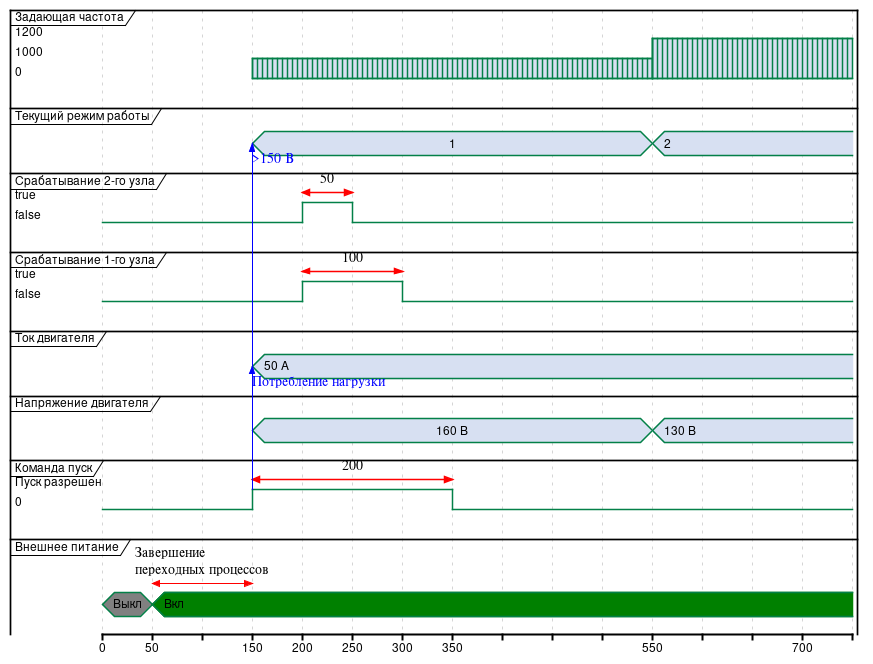
\includegraphics[height=.8\textheight,keepaspectratio]{modbus_scenario_example_diagram.png}
            \caption{Пример использования классов.}\label{fig:modbus_scenario_example_diagram}
        \end{figure}
    \end{center}
\end{landscape}


\section*{Выводы}
Таким образом можно использовать унифицированный способ представления сценария для имитатора \ldots



% \section{Распределение ролей}
% На стороне СК создается экземпляр клиента сети modbus,
% имитатор представляет сервер (см. главу \ref{ch:ch2}).
% \section{Конфигурационный файл}\label{sec:ch2/sec1}
% Общее пространство данных modbus у ПО СК и имитатора \ldots
% \section{Паттерн MVC}
% Поверх множества данных modbus используется паттерн проектирования модель-вид-контроллер \cite{book:pattern:band_of_4}.
% Библиотека Qt позволяет создавать модель данных, наследуя поведение от \lstinline[language=C]!QAbstractTableModel!,
% переобпределяя реализацию методов для чтения-записи данных в модель.
% \subsection{Пояснение в реализации методов}
% \subsection{Преимущества такого подхода}

